\documentclass[twocolumn, 12pt]{article}
\usepackage[utf8]{inputenc}
\usepackage[a4paper,
            left=0.75in,right=0.75in,top=1.2in,bottom=1.2in,%
            footskip=.25in]{geometry}
\setlength{\columnsep}{20pt}
\usepackage{float}
\usepackage{nccmath}
\usepackage{enumitem}
\usepackage{amsmath}
\setlength {\marginparwidth }{2cm}
%Includes "References" in the table of contents
\usepackage[nottoc]{tocbibind}

\providecommand{\keywords}[1]{\textbf{\textit{\\Keywords }} #1}
\title{COBRAS: A tool for analyzing the collaborative writing process including semantic analysis}
\author{
    Montero Lucia\\
    lucia.monterosanchis@epfl.ch
    \and
    Shengzao Lei\\
    shengzao.lei@epfl.ch
}
\date{\today}

\usepackage{graphicx}
\usepackage{xcolor}
\usepackage{todonotes}
\newcommand\lei[1]{\todo[inline, color=blue!30]{#1}}
\newcommand\lucia[1]{\todo[inline, color=yellow!40]{#1}}
\newcommand\anyone[1]{\todo[inline, color=orange!30]{#1}}

\newcommand\newtodo[1]{\todo[inline]{#1}}
\usepackage{listings}
\usepackage{inconsolata}
\definecolor{pgreen}{rgb}{0,0.5,0}
\definecolor{keyword}{HTML}{A71D5D}
\definecolor{emphco}{HTML}{008040}
\lstset{aboveskip=3mm,belowskip=3mm,numbers=left,numbersep=8pt,numberstyle=\small\ttfamily\color{gray},columns=flexible,showstringspaces=false,tabsize=4,showspaces=false,showtabs=false,breaklines=true,showstringspaces=false,breakatwhitespace=true,keepspaces=true,stepnumber=1,captionpos=t,escapeinside={<@}{@>},commentstyle=\color{pgreen},keywordstyle=\color{keyword},stringstyle=\color[HTML]{0086B3},basicstyle=\ttfamily,emphstyle=\color{emphco},upquote=true,literate={*}{{\char42}}1{-}{{\char45}}1{^}{{\char94}}1
}

\begin{document}
\maketitle

\begin{abstract}
  This report covers the work done during the semester projects of L. Montero and S. Lei under the supervision of S. Håklev at EPFL's CHILI lab.

  This work is based on the tool developed by L. Baligand and A. Pace. The aim of the project is to improve the previous analysis tool by including semantic analysis on the text and by introducing new heuristics that allow for a more relevant analysis of collaboratively written documents.
\end{abstract}

\keywords{Collaborative writing, FROG, online editors}

\section{Introduction}
  As stated by V. Southavilay et al., Collaborative Writing has received attention since computers have been used for word processing  \cite{southavilay2009writeproc}. The many tools available for collaborative writing make the collaboration process easier and have also modified the way in which collaborative text is produced. Particularly, in Education it has been noted that, when
  using computers, students prefer to make revisions while producing instead of after producing the text \cite{ref6}.

  The process of writing is crucial in determining the final text, hence the interest in analyzing this process in Education. Learning about the process of collaboratively writing a text can help us understand different aspects about the roles taken by collaborators (big text additions, small edits...) or how the general structure of the document changes in time (list-like paragraphs, regular paragraphs with a similar length, big semantic differences between paragraphs...), among others.

  This information can be used to identify the practices that can potentially lead to a good quality text - and the practices that may decrease the quality of a text. Defining the quality of a text is not in the scope of this project, as we focus on defining the heuristics that allow to correctly capture the relevant information about the writing process.

  It would also be useful to be able to do some predictions before the task is finished, using the information gathered about the writing process up until that moment, as a tool for teachers to know how well students are collaborating in time for correcting potential mistakes.

  COBRAS (COllaBorative pRocess Analysis with Semantics) allows to learn about collaboratively written texts by looking at the process of writing. The `S' in the name has been added because one of the characteristics of the tool is the use of Semantic Analysis.
  
  The tool and the data used for the current report have been previously used to obtain the results presented in the submission to the International Conference on Computer Supported Collaborative Learning (CSCL 2019) \cite{cscl19}.

\section{Data}
  The data we use to test our tool consists of a group of pads written by first year Economics students. They took part in an approximately 45 minute long writing session and were asked to work in pairs to complete a task.

The Pads obtained from these sessions include some documents produced during a shorter \textit{warm-up} writing session and there are some Pads that were written by a single author. These Pads have not been considered when carrying out some parts of the analysis.

\section{Architecture}
  The tool presented in this report is written in Python3 and the architecture (Figure \ref{Architecture_new}) is based on the one implemented by L. Baligand and A. Pace \cite{swisstext,FROG-analytics} (Figure \ref{Architecture}). 

  \texttt{ElementaryOperations}, \texttt{Operations} and \texttt{Paragraphs} have been kept the same as in the previous version of the tool:
  \begin{itemize}
    \item An \texttt{ElementaryOperation} represents a writing event and is defined by its position, timestamp, author and text to add or length to delete. It can be only be of type \texttt{add} or \texttt{del}.
    
    \item \texttt{Operations} consist of groupings of \texttt{ElementaryOperations}. They are classified in five different categories: write, delete, edit, paste or jump. \texttt{Operations} also have \textit{context information} that give more information about it. This context information is described in more detail in Section \ref{sub:operation_heuristics}.
    
    \item \texttt{Paragraphs} keep track of the lines in the text. Each \texttt{Paragraph} may represent either one line of text or one new line character. They are obtained by iterating over the \texttt{Pad}'s \texttt{ElementaryOperations} and identifying the line that they are modifying. The general idea is that inserting a new line character in the middle of an existing \texttt{Paragraph} results in three \texttt{Paragraphs}: the first part of the original one, a new line \texttt{Paragraph} and a third one representing the second part of the original \texttt{Paragraph}. This is explained in more detail in L. Balingand and A. Pace's report.
  \end{itemize}
  
      \begin{figure}[bhtp!]
        \centering
        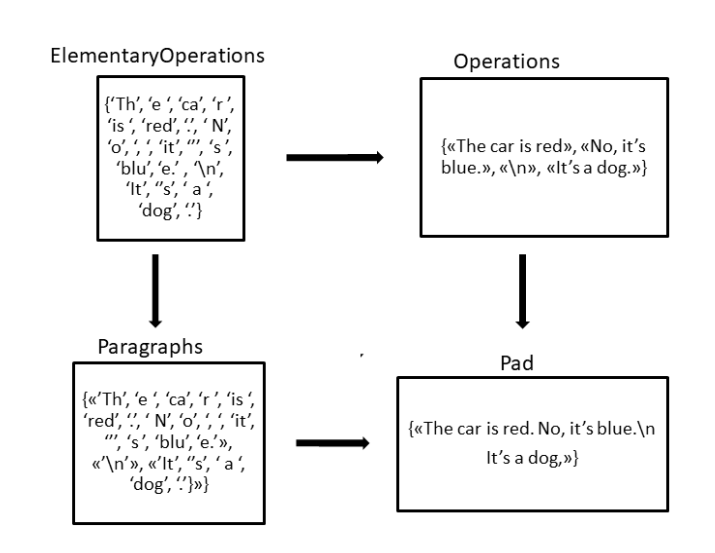
\includegraphics[width=0.5\textwidth]{figures/architecture.png}
        \caption{Architecture of the previous system}
        \label{Architecture}
    \end{figure}
    
    \begin{figure}[bhtp!]
        \centering
        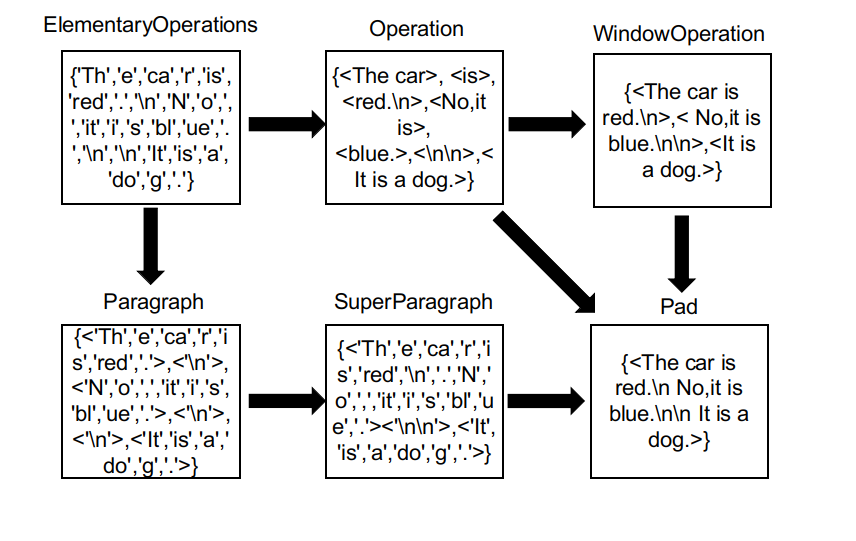
\includegraphics[width=0.5\textwidth]{figures/architecture-new.png}
        \caption{New architecture after adding \texttt{WindowOperation} and \texttt{SuperParagraph}}
        \label{Architecture_new}
    \end{figure}
  
  \newpage
  After reading the data, it is parsed to create \texttt{ElementaryOperations}. \texttt{ElementaryOperations} are grouped into \texttt{Operations}, which make up a \texttt{Pad}. \texttt{ElementaryOperations} are then used to deduce the \texttt{Paragraphs} of the document. Then, the heuristics are computed based on the Pads' paragraphs, operations and operations' context information.
  
  However, we realized that the majority of students use two new line characters (i.e. two new line characters written one after the other) to separate \textit{paragraphs}. In other cases students use  bullet points lists to synthesize information. Although a list's elements are separated by new lines, they should be considered part of one same structure - whereas different paragraphs should not. These observations lead us to introduce the concept of \texttt{SuperParagraphs}, which group several \texttt{Paragraphs}, keeping track of the fact that some \texttt{Paragraphs} are more related to some \texttt{Paragraphs} than to others. They are explained in Section \ref{sub:superparas}.

  We also introduce the concept of \texttt{Paragraph} indices and identifiers, which are explained in Section \ref{sub:para_ids}.
  
  Although we can obtain complete words from \texttt{Operations}, they are too fine-grained to contain a complete meaning and cannot be used to carry out the Semantic Analysis. Instead, we group the \texttt{Operations} with the same author and that take place within a specific time interval into a \texttt{WindowOperation}. A \texttt{WindowOperations} is defined by its group number (the group it belongs to), its author, the list of Operations it is composed of, its time interval and its starting and ending timestamp. \texttt{WindowOperation} are explained in Section \ref{sub:winOp}.

    \subsection{Paragraph indices and identifiers}
    \label{sub:para_ids}
    \textit{Paragraph indices} track the updated position of each text \texttt{Paragraph} in the \texttt{Pad}, and are useful to know the absolute position of the line or lines that have been modified by each \texttt{Operation}. 
    
    This information can be used to determine if consecutive \texttt{Operations} modify the same lines of the text, but a \texttt{Paragraph}'s index does not necessarily identify the same \texttt{Paragraph} at different points in time. It is interesting to keep track of how \texttt{Paragraphs} are split or merged, how the meaning of a \texttt{Paragraph} changes or where are the new \texttt{Paragraphs} introduced - for this, we introduce \textit{Paragraph identifiers (IDs)}.
    
    \subsubsection{Paragraph indices}
      \textit{Paragraph indices} are assigned to \texttt{ElementaryOperations} to keep track of the modified \textit{lines}' position in the text. With \textit{line} we refer to a text \texttt{Paragraphs}, as some \texttt{Paragraphs} only contain a new line and are not taken into account when computing paragraph indices.
      
      The position of a line is computed as the position of the text \texttt{Paragraph} in the \texttt{Pad} minus the number of newlines from the beginning until the position of the text \texttt{Paragraph}. Therefore, the paragraph index $i_p$ of a line that corresponds to the text \texttt{Paragraph} in position $p$ in the \texttt{Pad} would be computed as:
      \begin{equation}\label{eq:paraindex}
               i_p = p-\text{nl}(0,p-1)
      \end{equation}
      where nl$(p,q)$ is the number of \texttt{Paragraphs} in the \texttt{Pad} between positions $p$ and $q$ (both included) that are new line \texttt{Paragraphs}.
      
      Paragraph indices assigned to \texttt{ElementaryOperations} can give us an insight on whether the changes of an \texttt{Operation} are being done in the same part of the document as the previous or next \texttt{Operations}, or in a different part.
      
      Some questions that indices can give an answer to are: \textit{Is an author modifying one line of text or several ones? Are these lines close to each other? Are several authors working in the same  text area?}
      
      Paragraph indices are assigned with the object function \texttt{ElementaryOperation.assign}\_\texttt{para}, which is called by \texttt{Pad.create\_paragraphs\_from\_ops} while \texttt{Paragraphs} are created.
      
      When one or more \texttt{Paragraphs} are added or deleted entirely, the indices of other \texttt{Paragraphs} need to be updated. Ideally, when verifying if two consecutive \texttt{ElementaryOperations} EOperation1 and EOperation2 happen in the same part of the text we would compare EOperation1's indices (after updating the indices with EOperation1's changes) and EOperation2's indices (before updating the indices with EOperation2's changes). Therefore we need to distinguish between the indices before updating the \texttt{Paragraph} indices and the indices after updating the \texttt{Paragraph} indices.
      
      Moreover, some \texttt{ElementaryOperations} may modify several consecutive \texttt{Paragraphs}, so we define an \texttt{ElementaryOperation}'s paragraphs indices as two arrays of paragraphs indices (the first one for the paragraph indices \textbf{before} taking into account the \texttt{ElementaryOperation}'s changes, and the second one for the paragraph indices \textbf{after} taking into account the \texttt{ElementaryOperation}'s changes).
      
      For example, inserting a new text \texttt{Paragraph} in the beginning of the document shifts the index of all \texttt{Paragraphs} and index 0 would start being used by the newly inserted \texttt{Paragraph}. The indices assigned to the  \texttt{ElementaryOperation} that adds a new paragraph in the beginning of the text would be:
      \begin{itemize}
          \item \textbf{Before} changes: [0]\\
          We will insert the text line in the beginning, that is, next to line 0 - if we insert it between two existing lines, this array will contain both lines' indices.
          \item \textbf{After} changes: [0]\\
          We just inserted paragraph 0.
      \end{itemize}
      
      The rules applied to assign a Paragraph index to an \texttt{Elementary Operation} are shown in Table \ref{tab:eo_indices}. The definition of $i_p$ is the one from Equation \ref{eq:paraindex}. $N$ represents the position of the last \texttt{Paragraph} in the \texttt{Paragraph} array, which may be a new line or text depending on the case. $p$ is the position where we insert the new \texttt{Paragraph}.

      \begin{table}[htp]
        \caption{Paragraph indices assigned to an  \texttt{ElementaryOperation} - which always affects exactly one paragraph.}
        \label{tab:eo_indices}
        \centering
        \resizebox{\columnwidth}{!}{%
        \begin{tabular}{lrr}
            \hline
            \textbf{Elem. Operation} & \textbf{i before} & \textbf{i after} \\
            \hline
            \multicolumn{3}{l}{\textbf{Add text to existing text paragraph at \textit{p}}} \\
            ($0\leq p\leq N$)  & [$i_p$]                & [$i_p$]   \\
            \hline \multicolumn{3}{l}{\textbf{Add a new text paragraph at \textit{p}}} \\
            Beginning ($p=i_p=0$)       & [0]                & [0]   \\
            End ($p=N+1$)         & [$i_{N}$]         & [$i_{N+1}$]   \\
            Middle ($0<p\leq N$) & [$i_p$, $i_p$+1] & [$i_p$+1]             \\
            \hline \multicolumn{3}{l}{\textbf{Add a new new-line paragraph at \textit{p}}} \\
            Beginning ($p=0$)       & [0]                & [0]   \\
            End ($p=N+1$)         & [$i_{N}$]         & [$i_{N}$]   \\
            Middle ($0<p\leq N$) & [$i_{p}$, $i_{p}$+1] & [$i_{p}$, $i_{p}$+1]\textbf{}             \\
            \hline
            \multicolumn{3}{l}{\textbf{Add new-line in existing text paragraph at \textit{p}}} \\
            ($0\leq p\leq N$)  & [$i_p$]                & [$i_p$, $i_p$+1]   \\
            \hline \multicolumn{3}{l}{\textbf{Delete paragraph at \textit{p}}}\\
            Beginning ($p=i_p$=0)        & [0]               & [0]   \\
            End ($i_p=i_{-1}$)  & [$i_{-1}$]   & [$i_{-1}$-1]   \\
            Between $i_p$-1 and $i_p$+1     & [$i_p$]   & [$i_p$-1, $i_p$]             \\
            \hline
        \end{tabular}
        }
      \end{table}
      
      Since we are interested in knowing the paragraph indices for \texttt{Operations}, we compute them based on the paragraph indices that have been assigned to the \texttt{Operation}'s \texttt{ElementaryOperations}. The computation is carried out by the object function \texttt{Operation.get\_assigned\_para}, which receives two arguments: whether we are interested in the paragraphs before or after applying the changes and whether we want the first or the last paragraph involved.
      
    %   Variable \textbf{paragraph} refers to the \texttt{Operations}' Paragraph index that corresponds to picking the first paragraph modified and in the order in which they were before the modification.

    \subsubsection{Paragraph IDs}
        \label{subs:paraids}
    Although it is not being used at the moment, it is interesting to keep track of how \texttt{Paragraphs} are modified, split or merged or where new \texttt{Paragraphs} are introduced. For this purpose we introduce \textit{Paragraph identifiers} (\textit{Paragraph IDs}).
      
    Paragraph \textit{IDs} are computed by looking at the \texttt{Pad}'s array of all \texttt{Paragraphs} - which contains the \texttt{Paragraphs} that have been deleted as well as the ones that currently exist. This way we make sure that IDs are unique.
      
     This functionality is implemented in the class function \texttt{Operation.compute\_para\_id}. This function receives as parameters: one or two existing IDs that will be used to compute the new ID (or IDs, in some cases) and the \textit{relation} between the new and the reference paragraphs.
      
      The possible values of \texttt{relation} are {initial}, {merge}, {split}, {insert\_before}, {insert\_after} and {insert\_between}. The value of the new ID or IDs based on the parameter \texttt{relation} are:
      \begin{itemize}
        \item \texttt{initial}: The first ID is always 0.
        \item \texttt{insert\_before (id)}: Paragraph is inserted in the beginning of the text or when inserting a paragraph between two paragraphs if the second one has a shorter ID than the first one.\\
        Examples:\\
        \{0 $\rightarrow$ -1\}; 
        \{-1 $\rightarrow$ -2\}; 
        \{2 $\rightarrow$ 1\}; \\
        \{1 $\rightarrow$ 0\}; 
        \{0.A.B\_1\_3 $\rightarrow$ -1\}

        \item \texttt{insert\_after (id)}: Paragraph is inserted in the end of the text or when inserting a paragraph between two paragraphs if the first one has a shorter ID than the second one. Examples:\\
        \{-1 $\rightarrow$ -1\_0\};
        \{0 $\rightarrow$ 0\_0\};
        \{0\_2 $\rightarrow$ 0\_3\}
        \item \texttt{merge (id1, id2)}: Lastly, we can obtain a new ID for a paragraph that results from merging two previously existing paragraphs. Examples:\\
        \{0, 1 $\rightarrow$ (0+1)\};
        \{0.A, 0.B $\rightarrow$ 0.A\};\\
        \{0.C, 0.D $\rightarrow$ 0.C\};\\
        \{0.A, 0.C $\rightarrow$ (0.A+0.C)\};\\
        \{0.A.B, 0.A.C $\rightarrow$ 0.A.B\};\\
        \{0.A, 0.B.C $\rightarrow$ (0.A+0.B.C)\}
        \item \texttt{insert\_between (id1, id2)}: Paragraph is inserted between two paragraphs. It compares the lengths of both IDs and inserts the new one either before id2 or after id1. For example, the paragraph inserted between 0 and 1 is 0\_0.
        \item \texttt{split (id1)}: If an existing paragraph is split into two, three IDs are generated from the original ID. For example, splitting paragraph 0 results in\\0.A (text), 0.B (new line) and 0.C (text).
      \end{itemize}
    
    These IDs are called \textbf{Paragraph History}. However, for when we want to see if two users have contributed for the same paragraph or not, we can use the variable \textbf{Paragraph Original}. Paragraph Original is computed based on Paragraph History, but it considers paragraphs 0.A, 0.B, 0.C all as paragraph 0. Also, it would consider paragraph (0+1) as paragraph 0. We can increase the complexity, for example, paragraph history ((0.C+1).C+4) would become paragraph original number 0. 

    One of the problems that we identified with this implementation of Paragraph IDs is that in some cases IDs become very long. For this reason, when the paragraph ID is longer than the maximum length specified in \texttt{config.py}, we generate a completely new ID - sort of \textit{restarting} the ID to a short length again. This solution is not very convenient, as the analysis becomes more difficult.
    
    A possible solution for this would be to come up with a way to track how many parts a paragraph has been split into. With the current implementation, if we decide to merge paragraphs 0.A and 0.B we cannot be sure if the result should be 0 (which would be the case if 0=(0.A+0.B), i.e. there are no paragraphs 0.C, etc), or if paragraph 0 was split into more than 2 parts and therefore (0.A+0.B) would only be a part of paragraph 0.
    
    Using SuperParagraph IDs (the concept of a SuperParagraph is introduced in the next section)  instead of Paragraph IDs would also reduce the length of the IDs used, but the implementation is a bit less straightforward. However, a simplified version has been implemented.

  \subsection{{SuperParagraphs} and {Paragraphs}}
    \label{sub:superparas}
    In this version of the tool we introduce the concept of \texttt{SuperParagraph} that groups several \texttt{Paragraphs} if certain conditions are met. \texttt{SuperParagraphs} allows to keep track of the likely relationship that exists between lines of text that are only separated by one new line character.
    
    \texttt{SuperParagraphs} contain a boolean that states whether the \texttt{SuperParagraph} consists of only new lines or not, which could be understood (in a simplied way) as the result of doing the logical AND operation of the boolean that states whether each of the \texttt{SuperParagraph}'s \texttt{Paragraphs} are new lines. Hence, this boolean defined for \texttt{SuperParagraphs} determines the possible \texttt{Paragraphs} that it can contain. 
    \begin{itemize}
        \item New line \texttt{SuperParagraph}:\\
        It may contain any number $N\geq 2$ of new line \texttt{Paragraphs}.\\
        There cannot be two new line \texttt{SuperParagraphs} one after the other, as in that case they should be merged. Therefore, a new line \texttt{SuperParagraph} can only be surrounded by text \texttt{SuperParagraphs}.
        \item Non-new line (\textit{text}) \texttt{SuperParagraph}:\\
        It may contain any number of \texttt{Paragraphs}, either text or new line, as long as there are not two (or more) new line \texttt{Paragraphs} one after the other.\\
        Analogously to the previous case, they can only be surrounded by new line \texttt{SuperParagraphs}.
    \end{itemize}
    
    Object function \texttt{Pad.create\_paragraphs\_ from\_ops()}, which is the function that updates \texttt{Paragraphs}, is the one that updates \texttt{SuperParagraphs} as well.
    
      \begin{table}[htp]
        \caption{Rules for updating \texttt{SuperParagraphs} after inserting or deleting a \texttt{Paragraph}. \textbf{NL} stands for \textit{New Line} and \textbf{T} stands for \textit{Text}.}
        \label{tab:sup_paras}

        \centering
        \resizebox{\columnwidth}{!}{%
        \begin{tabular}{lll}
            \hline
            \textbf{Para} & \textbf{SuperPara} & \textbf{Action} \\
            \hline
            Any & None & Insert in new T SuperPara \\
            T & NL & Insert; Run Listing \ref{code:code2} \\
            T & T & Insert\\
            NL & NL & Insert \\
            NL & T & Insert; Run Listing \ref{code:code1}\\
            \hline
        \end{tabular}
        }
      \end{table}
    
    The rules that determine how to update \texttt{SuperParagraphs} after inserting or deleting a \texttt{Paragraph} are shown in Table \ref{tab:sup_paras}. 

    After inserting a text \texttt{Paragraph} in a new line \texttt{SuperParagraph} we also need to check which are the changes that we will need to do in the \texttt{SuperParagraph}, as described in Listing \ref{code:code2}.
    \lstinputlisting[language=Python, caption=After inserting text Paragraph in new line Superparagraph., label=code:code2]{codes/Tpara.py}    

    In a similar way, after inserting a new line \texttt{Paragraph} in a text \texttt{SuperParagraph} we need to check whether we will need to split the \texttt{SuperParagraph} or merge it with other \texttt{SuperParagraphs}, as described in Listing \ref{code:code1}.
    \lstinputlisting[language=Python, caption=After inserting new line Paragraph in text Superparagraph., label=code:code1]{codes/NLpara.py}

    \subsubsection{Discussion about SuperParagraphs: Issues and possible solutions}
      Although using \texttt{SuperParagraphs} seems to work for the majority of the pads analyzed, there is still an inconsistency in the number of new line characters used to separate paragraphs. In some cases, both the separation between paragraphs and the separation between list elements is one new line character. This makes it difficult to apply the concept of \texttt{SuperParagraphs} - at least with the current implementation. These cases can be identified by a small number of \texttt{SuperParagraphs} and a very large average number of \texttt{Paragraphs} per \texttt{SuperParagraph}. A possible improvement for these cases would be to assume \texttt{SuperParagraphs} to be the same as the \texttt{Paragraphs}, unless there seems to be a list (which can be identified by having several short \texttt{Paragraphs} that often start with one of the characters that are typically used for lists).
      
      A correct paragraph separation was crucial at this point for carrying out a relevant semantic analysis comparison across paragraphs. For this reason, we have implemented the object function \texttt{Pad.get\_paragraphs\_text()} that first obtains the text split by double new lines and then compares the average paragraph length obtained with a configuration parameter that we considered appropriate for the texts we are analyzing (1000 characters, defined in the configuration file \texttt{config.py}). If the average length is longer than the one defined in the configuration file, we assume that the authors used single new line characters to separate their paragraphs and split the text by single new lines instead. In both cases we delete whitespace lines.
      
      Another issue that we came up with when dealing with \texttt{SuperParagraphs} is the fact that lines consisting only of whitespace are considered as text \texttt{Paragraphs}, and therefore we may end up grouping in a single \texttt{SuperParagraphs} lines of text that the authors intended to separate in different paragraphs. The solution to this is in the way \texttt{Paragraphs} are treated: whitespace \texttt{Paragraphs} behave like text \texttt{Paragraphs} when being updated, but should be considered like new line \texttt{Paragraphs} when grouped into \texttt{SuperParagraphs}. This is not completely straightforward, as a \texttt{SuperParagraph} containing a whitespace \texttt{Paragraph} may need to be split and recombined if non-whitespace characters are inserted in its whitespace \texttt{Paragraph}.
      
      Another of the issues we identified happens as a result of the behaviour of many text editors that automatically insert a new bullet point after inserting a new line character in a line with a bullet point. In many cases, authors leave this new bullet point entry empty - using it as if it were an empty line - but our program considers it as a line containing text.
  \subsection{WindowOperation}
    \label{sub:winOp}
    A \texttt{WindowOperation} is a group of \texttt{Operations} within a time interval that have the same author. We introduced \texttt{WindowOperations} because we would like to apply semantic analysis on what users' wrote and sometimes we can only obtain one or two words from \texttt{Operations},  not enough to constitute meaning. 
    
    \subsubsection{Build WindowOperation}
    Function \texttt{Pad.BuildWindowOperation} creates the \texttt{WindowOperation}. It takes \texttt{time\_interval} (default 100 second) as a parameter, which needs to satisfy some conditions that we will explain later. The function traverses all \texttt{Operations} inside the pad and computes their group number, which is then used to assign each \texttt{Operation} to its corresponding group. Within each group,  \texttt{Operations} are sorted and split by author, resulting in  \texttt{WindowOperations}. The group number (num) can be computed as:
        \begin{equation}\label{eq:group_number}
            \text{num} = \lceil(\text{end\_time} - \text{start\_time})/t\rceil
        \end{equation}
      where $t$ is the time interval, end\_time is time when the \texttt{Operation} ends and start\_time is the starting time of the \texttt{Operation}'s Pad.

      \subsubsection{Select time interval}
      \label{sub:time_interval}
      Function \texttt{BuildWindowOperation} uses parameter time\_interval, which has a great impact on applying semantic analysis. Too short time interval may lead to not having enough words that have a meaning, whereas too long time interval may result in not having enough points in time for analyzing of collaborative writing behavior in time.
      
      We first tried to choose the best time interval by counting the number of \texttt{Operations} or string length inside one \texttt{WindowOperation}, but we found that there are some \texttt{Operations} which only add a new line or punctuation. Since we would like to do semantic analysis to the \texttt{WindowOperation}'s text, we are interested in the \texttt{WindowOperation}'s meaningful text and these \texttt{Operations} should not be considered. Therefore, it makes sense to evaluate the best time interval by counting the number of words inside the \texttt{WindowOperation}. We consider a \texttt{WindowOperation} to be valid if it has enough words. A \texttt{Pad} is considered valid if the \texttt{Pad} has enough valid \texttt{WindowOperations}. Function \texttt{SelectTimeInterval} labels whether the  \texttt{Pad} is valid or not for a given list of time intervals to be considered. It also takes the threshold number of words needed for a valid \texttt{WindowOperation} and the threshold of the group number in a \texttt{Pad} as parameters. It returns, for each \texttt{Pad}, a list containing the 0 and 1 (valid) of \texttt{Pad} for each time interval.

      \subsubsection{Fitting similarity distribution} Users' behavior is quite complex when they are writing together. However, we can simplify collaborative behavior by using some metrics to measure it and try to discover potential common patterns. After choosing a time interval and building the corresponding \texttt{WindowOperations}, we can recover the text (see Section \ref{sub:textRecovery} for more details) and apply a pre-trained model (Section \ref{sub:pretrained}) to compute the similarity (see Section \ref{sub:similarity}) between different authors' \texttt{WindowOperations} in the same group. From here on we will refer to the different authors' \texttt{WindowOperations} in the same group call as \texttt{WindowOperation} pair. After obtaining the sequence of similarity values for all \texttt{Pads} and for each authors pair, we can plot the similarity distribution and fit the similarity distribution, to find the pattern or the \textit{law of similarity}. We used linear fitting to fit similarity distribution, so that we can classify the collaborative behaviours in: 
      \begin{itemize}
          \item Writing converges towards the same topic gradually.
          \item Writing topic diverges gradually.
          \item No change in the writing topic similarity.
      \end{itemize}
      Function \texttt{PlotSimilarityDistribution} takes care of fitting similarity distribution.
    
    
% \newpage
\section{General Heuristics Computation}
      There have been many different approaches for analyzing Collaborative Writing (CW). Although most of the research has been traditionally done on the final result, there have been several approaches that focus their analysis on the process of writing. In particular, the WriteProc framework presented by V. Southavilay et al. in uses both process mining and semantic analysis \cite{southavilay2009writeproc}.
    
    Lowry et al. present in \cite{lowry2004building} a common nomenclature and taxonomy for CW works. They define the common iterative activities of CW, which are: brainstorming, outlining, drafting, reviewing, revising and editing. Several participants' roles are introduced by Lowry et al. in \cite{lowry2004building} as well, including writer, editor, scribe or facilitator. Depending on the task that students are working on, some of these activities and roles may not be relevant. In our case, it is very unlikely to find a student taking the role of scribe, as all interaction was done through the computer. Nevertheless, we would expect students to often take the roles of writer and editor. For a similar reason, we would not be able to find the reviewing activity either.
    
    In this section we will define different heuristics and measures that may help us identify different roles taken by students or different collaborative activities, that we might be able to relate to the ones proposed by Lowry et al. For example, as explored in \cite{sv2}, an increase in the number of lines together with a decrease in the length of such lines could suggest an outlining activity.
    
    There are many other specific questions that we may want to answer, such as which areas of text have been modified the most, if students have worked at the same time, or whether several students have contributed to the same parts of the document. The heuristics that were proposed in the previous version of our tool \cite{FROG-analytics} contained some information that could be relevant for some of these questions, but we can see that other researchers have been interested in this topic as well \cite{sv3}.

\subsection{Pad heuristics}
\label{sub:Pad_heuristics}
    In the previous version of the tool \cite{FROG-analytics} the heuristics or metrics that are summarized in Table \ref{tab:pad_h} were defined in order to assess the quality of a \texttt{Pad}. From here on, we refer to this kind of heuristics as \textit{Pad heuristics} because they are computed taking into account the \texttt{Pad}'s \texttt{Operations}, as opposed to \textit{Operation heuristics} that will be introduced in the next section.
    
      \begin{table}[htp]
        \caption{Pad heuristics. Column \textit{Window} indicates whether the scores can be computed ignoring Operations before a given timestamp.}
        \label{tab:pad_h}
        \centering
        % \resizebox{\columnwidth}{!}{%
        \begin{tabular}{lll}
            \hline
            \textbf{Heuristic name} & \textbf{Window} & \textbf{} \\
            \hline
            Alternating & No & \\
            Day break & Yes & \\
            Short break & Yes & \\
            Overall type & Yes & \\
            Proportion & No & \\
            Synchronous & Yes & \\
            User type & Yes & \\
            User proportion per paragraph & No & \\
            \hline
        \end{tabular}
        % }
      \end{table}
    We can compare the scores of a \texttt{Pad}'s heuristics at different points in time by getting versions of the \texttt{Pad} at the timestamps of interest, using the object function \texttt{Pad.pad\_at\_timestamp}. When calling function \texttt{run\_analytics.py} with argument \texttt{--generate\_csv\_summary} a tsv file is printed containing one line per \texttt{Pad} with the values of the previous and new \textit{Pad heuristics}. These Pad heuristics are computed by calling the object function \texttt{Pad.compute\_metrics}.
 
    The metrics implemented in the previous version of the tool take into account all \texttt{Operations} within a \texttt{Pad}, from the first timestamp until the last one. However, these scores \textit{dilute} the impact of each \texttt{Operation} because, as the number of \texttt{Operations} in the \texttt{Pad} increases, the new \texttt{Operations} have a smaller impact on the scores.

    To solve this issue, we can specify a starting timestamp so that \texttt{Operations} that take place before the specified time are not taken into account when computing the scores. This, together with the previously explained strategy of getting versions of the \texttt{Pad} that end at different timestamps, allows us to define time windows of interest. This can be applied to the scores that are computed from the \texttt{Pads}' \texttt{Operations}, but not to the ones computed from \texttt{Paragraphs} information. Table \ref{tab:pad_h} summarizes which scores can be computed for specific time windows.

    We also defined some new heuristics that capture \texttt{Paragraphs} information in a different way. These new pad heuristics are summarized in Table \ref{tab:new_pad_h}.
      \begin{table}[pth!]
        \caption{New Pad heuristics (not normalized). Column \textit{Wnd} (Window) indicates whether they can be computed ignoring Operations before a given timestamp.}
        \label{tab:new_pad_h}
        \centering
        \resizebox{\columnwidth}{!}{%
        \begin{tabular}{lll}
            \hline
            \textbf{Heuristic name}&\textbf{Wnd} & \textbf{Details}\\
            \hline
            Length & No & Contribution\\
            Length all & Yes & Contribution\\
            Length all write & Yes  & Student effort \\
             & & and contribution \\
            Length all paste & Yes  & Contribution\\
            Added chars &  Yes & Contribution\\
            Deleted chars &  Yes &Contribution \\
            Para avg length & No & Text structure\\
            Superpara avg length & No & Text structure\\
            Avg paras per superpara & No & Text structure\\
            \hline
        \end{tabular}
        }
      \end{table}
    
  \subsection{Operation heuristics}
    \label{sub:operation_heuristics}
    As mentioned previously,  \texttt{Operation} heuristics only take into account the context of the \texttt{Operation}. They are shown in Table \ref{tab:op_h}, together with other relevant information.

      \begin{table}[pth!]
        \caption{Operation information (heuristics not normalized).}
        \label{tab:op_h}
        \centering
        \resizebox{\columnwidth}{!}{%
        \begin{tabular}{ll}
            \hline
            \textbf{Information} & \textbf{Details} \\
            \hline
            Author & Name of the Operation author.\\
            Position Start & First text position edited.\\
            Position End & Last text position edited.\\
            Time Start & Operation starting timestamp.\\
            Time End & Operation ending timestamp.\\
            Atomic Op Count & Number of atomic ops.\\
            Type & Operation type.\\
            Text Added & Number of chars. added.\\
            Deletion Length & Number of chars. deleted.\\
            Paragraph & Paragraph index.\\
            Paragraph History & Paragraph ID, see \ref{subs:paraids}) \\
            Paragraph Original & Simplified Para. ID, see \ref{subs:paraids}) \\
            Superparagraph ID & Computed as in \ref{subs:paraids}. \\
            Coauthor Number & Number of other authors \\
            & in SuperParagraph.\\
            Proportion Pad & Ratio of Operation chars\\
            & to Total Pad chars.\\
            Proportion Paragraph & Ratio of Operation chars\\
            & to Paragraph chars. \\
            \hline
        \end{tabular}
        }
      \end{table}

\section{Semantic Analysis}
  When analyzing students' collaborative behaviour, the meaning of what they are writing can give us very useful insights. In order to apply machine learning algorithms to obtain these insights into the semantic information of the texts or in order to project the text into a latent d-dimensional space we need to use semantic analysis.
 \subsection{Pre-trained models}
 \label{sub:pretrained}
 Due to the relatively small size of our data, as well as computational constraints and time limitations, it would be impossible for us to build a good performance model. However, there are many pre-trained models available, which have already been trained on large datasets and make semantic analysis faster and less expensive (data and computation-wise).
 
 There are several pre-trained models available online that have been shared by different Machine Learning research groups. We chose three different pre-trained models and compare their performance on our dataset.
 
 \subsubsection{doc2vec}
 Le and Mikolov proposed doc2vec as a extension to word2vec to learn document-level embeddings \cite{doc2vec}. Then, Jey Han and Timoth verified doc2vec model's performance by comparing it to two baselines and two state-of-the-art document embedding methodologies and shared their pre-trained models \cite{doc2vecPretrained}. We downloaded two pre-trained doc2vec (DBOW method) models that have been trained on the English Wikipedia and Associated Press News websites respectively. 
\subsubsection{sent2vec}
A novel, computationally efficient, unsupervised, C-BOW-inspired method was introduced by Matteo and approach for training and inferring sentence embedding\cite{sen2vec}. We use two of their pre-trained sent2vec models, which were trained on the English Wikipedia and Toronto books respectively.
\subsubsection{Spacy}
Spacy is an open-source python library for industrial-strength natural language processing. It offers several pre-trained models such as \textit{en\_core\_web\_lg}, which is an English multitask CNN trained on OntoNotes, with GloVe vectors trained on Commom Crawl.
\subsection{Test Dataset}
In order to compare the performance of each pre-trained model on our dataset, we manually select some data as the test dataset and split it into three groups of text pairs depending on whether we considered them to be similar, medium similar or non-similar to each other. The text pairs of similar data were created by translating English text into Chinese and then translating Chinese to English. As for non-similar data and medium similar data, the text pairs are selected from each document of our dataset.
\subsection{Data Preprocessing}
There are many characters and groups of characters that are useless for semantic analysis such as punctuation, whitespace, very common words, numbers, URLs and so on in the text. Function \texttt{cleanedText} removes common words (Stoplist in Spacy), punctuation characters, numbers and URLs, then changes everything to lowercase and stores the prototype of each word. In addition, we defined different text processes that were applied to the text after our first processing, that were necessary for using the pre-trained models afterwards because of each pre-trained model's special requirements.
\subsection{Text Recovery}
\label{sub:textRecovery}
Recovering text based on \texttt{WindowOperation}, \texttt{SuperParagraph} or \texttt{Pad} is the most essential step before we do semantic analysis and we will use recovery text in \texttt{WindowOperation} as expample in following introduction. Recovering text is quite difficult in \texttt{WindowOperation} since we separated Operations by authors when creating \texttt{WindowOperations} from \texttt{Pad}, and collaborators' interaction information between cannot be retained. For example, when user1 wrote `year' in one \texttt{Operation} and user2 found this word should be plural form and then user2 add a \texttt{Operation} which added `s' at the end of `year'. This interaction is ignored when we only record one author's \texttt{Operations} in one \texttt{WindowOperation}. Fortunately, this kind of situation only happened by chance and it does not have a great impact on sentence embedding when we have enough words in one \texttt{WindowOperation}. In the beginning we tried to recovery text by \texttt{ElementaryOperation}, in which we needed to real-time trace the position of each \texttt{ElementaryOperation}. And tracing \texttt{ElementaryOperations}' position is not easy since you do not have completed position change information.  For example, the recovered text will be wrong in use1's \texttt{WindowOperation} when use2 modified(add or delete) a letter in the medium of text, since the \texttt{ElementaryOperations}' position is based on total \texttt{Pad} and user1 do not have user2's \texttt{ElementaryOperations}' information when two users \texttt{ElementaryOperation} are in different \texttt{WindowOpeartions}. Finally we tried to recover text base on \texttt{Operation} since we can obtain completed words from each \texttt{Operation}. We created a function \texttt{getOpText} to recover text and then sorted the \texttt{Operations} by start time and recover \texttt{WindowOperation}'s text by \texttt{Operation}'s text and its position. As for \texttt{Superparagraph}, function \texttt{pad\_at\_timestamp} creates a copy of a pad until a specific time and we can then retrieve the \texttt{Pad}'s text and separate it to obtain the superparagraphs' texts. Function \texttt{PreprocessOperationByAuthor} groups the \texttt{Operations} by authors and recovers their text, to see the similarity between different users in the total \texttt{Pad}.

\subsection{Similarity of WindowOperation and SuperParagraph}
After retrieving the text to be analyzed and choosing the  pre-trained model we can carry out the text analysis. We use cosine similarity between two vectors of texts, which is one of the most commonly used metrics for measuring similarity. When there is only one valid text in the pair, which means that there is only one non-zero text vector, we set the similarity value to 0. We apply the similarity metric on \texttt{WindowOperation} in order to find whether collaborators' writing topics tend to be gradually more similar. We will also look at the comparisons between \texttt{SuperParagraphs}.
\label{sub:similarity}


\section{Results}
We will select the best time interval based on the requirements for the Semantic Analysis and then we will keep the consistency by using the chosen value for the entire analysis.
  \subsection{Time interval selection}
Before selecting the best time interval we need to set two parameters: the threshold number of words in one \texttt{WindowOperation} and the threshold number of valid \texttt{WindowOperation} groups in one \texttt{Pad} (see Section \ref{sub:time_interval}). We set the minimum number of words to 10 according to the average length datasets STS2014-Forum (10.12 words), SICK2014 (9.67 words) \cite{sen2vec}. Also, in order to fit the similarity distribution we need enough similarity values in one \texttt{Pad}, so we set 5 as the minimum value of valid \texttt{WindowOperation} groups in a valid \texttt{Pad}. 
As we can see in Figure \ref{TimeInterval}, the candidate time intervals are from 60s to 380s. We chose 180s as it is the time interval with the most valid \texttt{Pads}.
\begin{figure}[htp]
    \centering
    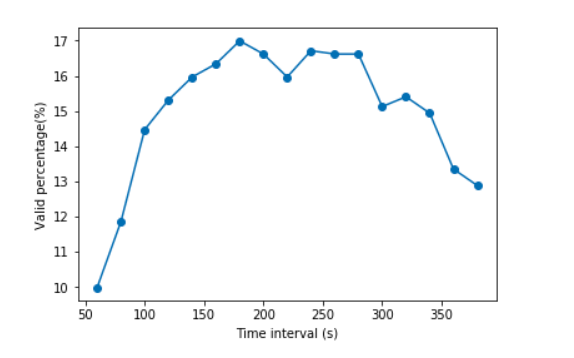
\includegraphics[width=0.5\textwidth]{figures/select_time_interval.png}
    \caption{Valid \texttt{Pad} percentage for different time interval durations}
    \label{TimeInterval}
\end{figure}

\subsection{Heuristics Analysis}
    We first look at the effect of considering only Operations after a specific start timestamp for computing \texttt{Pad} heuristics and compare it  to the score that considers \texttt{Operations} from the start. Then we see how \texttt{Paragraph} number and \texttt{Superparagraph} length evolve in time and we use time series analysis to see whether we could use these metrics to predict how much longer the students will take to finish the task.
    \subsubsection{Comparison between full Pad and window scores}
        We presented the need for modifying the scores that we were computing in the previous version of the tool so that the changes introduced by new \texttt{Operations} have a more noticeable impact.
        However, we need to keep in mind that some \texttt{Operations} may not be considered when using the window-contained Operations approach, particularly if some \texttt{Operations} are not fully contained within a single time window.

        Figures \ref{fig:typeoverallscorewrite} and \ref{fig:windowtypeoverallscorewrite} show the overall scores for writing operations, both using the defined time interval of 3 minutes. These Figures show in gray the boxplots of the score values per window for all pads, and in blue the average value with the standard deviation error bars.
    
        \begin{figure}[htp!]
            \centering
            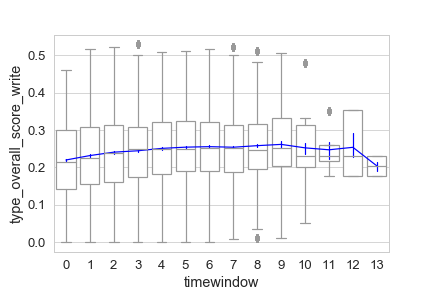
\includegraphics[width=0.5\textwidth]{figures/typeoverallscorewrite.png}
            \caption{Overall score for write type using 3 min time windows and considering Operations from the beginning of the Pad.}
            \label{fig:typeoverallscorewrite}
        \end{figure}
        \begin{figure}[htp!]
            \centering
            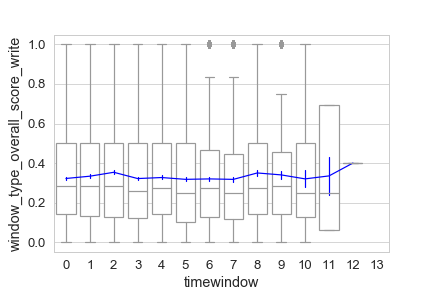
\includegraphics[width=0.5\textwidth]{figures/windowtypeoverallscorewrite.png}
            \caption{Overall score for write type using 3 min time windows and considering Operations from the beginning of the window (new implementation).}
            \label{fig:windowtypeoverallscorewrite}
        \end{figure}
        
        In Figure \ref{fig:typeoverallscorewrite} the line is smoother, as we are considering all the Operations from the beginning of the Pad until the end of the current window and therefore at every window we are averaging any possible changes with the rest of the Pad. Figure \ref{fig:windowtypeoverallscorewrite} shows the score changes from one window to another more clearly, as it is only considering the Operations within the time window. 
        
    \subsubsection{Paragraph and Superparagraph length in time} 
    In this section we decided to look at the number of paragraphs per superparagraph and at the average paragraph length and how these metrics change in time. We decided to try a simple model to see how well it could fit our data, and the results are shown in Figures \ref{fig:avg_p_sp} and \ref{fig:avg_len_p}. In both cases we decided to fit the values observed that correspond to windows 0 to 13, as windows 14 to 17 have less observations (because most paragraphs last 45 minutes or less, i.e. they last only 15 timewindows). However, we plot the results for windows 15 to 17 as well.
    
        \begin{figure}[htp!]
            \centering
            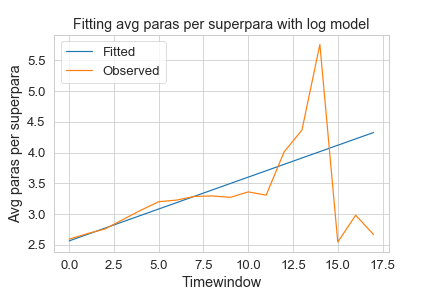
\includegraphics[width=0.5\textwidth]{figures/avg_p_sp.png}
            \caption{Average number of Paragraphs per Superparagraph. The linear model fitted has slope 0.1 and offset 2.55.}
            \label{fig:avg_p_sp}
        \end{figure}
        \begin{figure}[htp!]
            \centering
            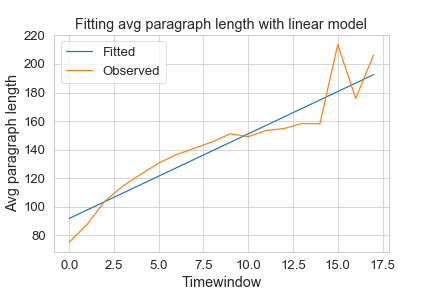
\includegraphics[width=0.5\textwidth]{figures/avg_len_p.png}
            \caption{Average length in characters per Paragraph. The linear model fitted has slope 5.9 and offset 91.8.}
            \label{fig:avg_len_p}
        \end{figure}
    
    From the two metrics obtained here we could obtain the value of the average Superparagraph length, as it would be the product of both.
    
    We see that the tendency does not seem to converge, so from these results we would not be able to say whether we could predict when the task will be finished. However, we need to keep in mind that the average for first windows has been computed over more pads than for the last windows. As we can see, up until timewindow 11 (which would correspond to minute 33 of the task), it seems like the values would converge. For this reason, it may be interesting to repeat this analysis after implementing a different WindowOperation split that takes into account the total duration of the pad.
\subsection{Semantic Analysis}
\label{sub:result_semantic}
Figure \ref{similar} shows the similarity value of three datasets. As we can see from those similarity values of each models for different similarity paragraph texts. \texttt{doc2vec} models can clearly recognize different similarity paragraph texts, but it has lower values even the the paragraph looks very similar and took the longest time to compute similarity. As for the fastest \texttt{spacy} model, it performed bad since the values of them are always very high even the two texts are totally different. And \texttt{sent2vec} model can correctly recognize them . Additionally, we can discover the different performances of those models when applying to same paragraph pair. \texttt{Spacy} model always have the highest values and  \texttt{doc2vec} always have the lowest values.  Overall, for each two paragraph pairs, the similarity difference(increase or decrease) between these two pairs are almost the same between different models. We finally chose \texttt{sent2vec} as our pre-trained model since it took less time and performed well in different similarity datasets.
    \begin{figure}[htp]
        \centering
        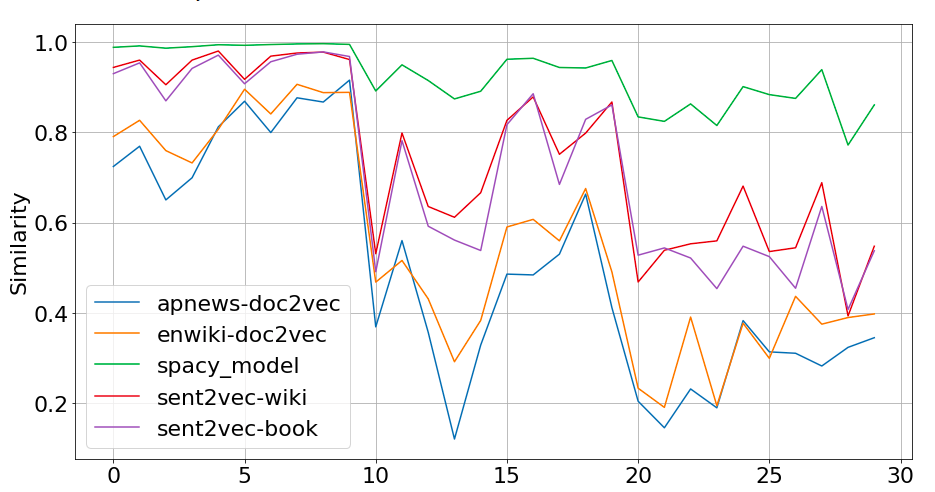
\includegraphics[width=0.5\textwidth]{figures/pre-trained-text.png}
        \caption{The evaluation similarity value of datasets}
        \label{similar}
    \end{figure}
    
\subsection{Fitting similarity distribution}
We could roughly separate our dataset into three categories depending on the trend of the semantic similarity distribution (increasing, stable and decreasing). However, at this point it is difficult to tell whether this classification would give us useful insights on the collaborative behavior  of the students.

Figure \ref{fitting} shows the similarity distribution of one valid \texttt{Pad}. We fitted a linear model to the observed data. From the Figure, we can easily see an increasing trend in topic similarity between this \texttt{Pad}'s authors, reflected in the positive slope of the fitted model. 

\begin{figure}[htp]
    \centering
    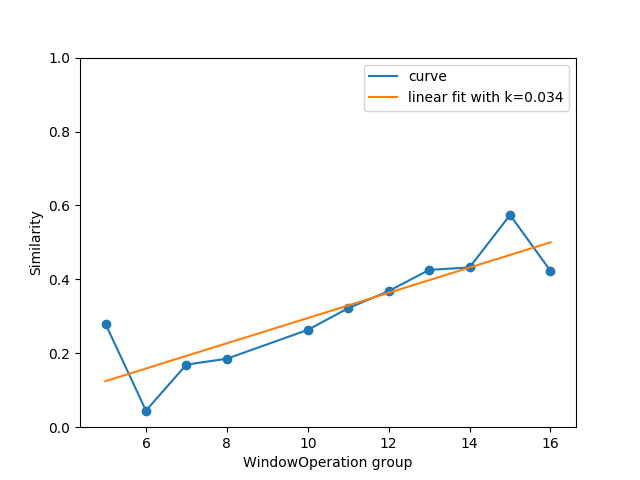
\includegraphics[width=0.5\textwidth]{figures/linear_fiting.png}
    \caption{Fitting similarity distribution}
    \label{fitting}
\end{figure}



\subsection{SuperParagraph similarity visualization}
When applying semantic analysis on \texttt{SuperParagraphs}, we first plot the heatmap for similarity values between all \texttt{SuperParagraphs} to get an overview of the document semantics. The heatmap in Figure \ref{similarity_heatmap} shows the inter \texttt{SuperParagraphs}' similarity in one document from our dataset.

We can conclude that \texttt{SuperParagraphs} 0 and 13 are the most different pair and \texttt{SuperParagraphs} 1 and 12 are the most similar pair. We include below the texts of those 4 \texttt{SuperParagraphs}, as it can be used to verify if we agree with the results and to get some intuition on how the results are computed:

\begin{figure}[htp]
    \centering
    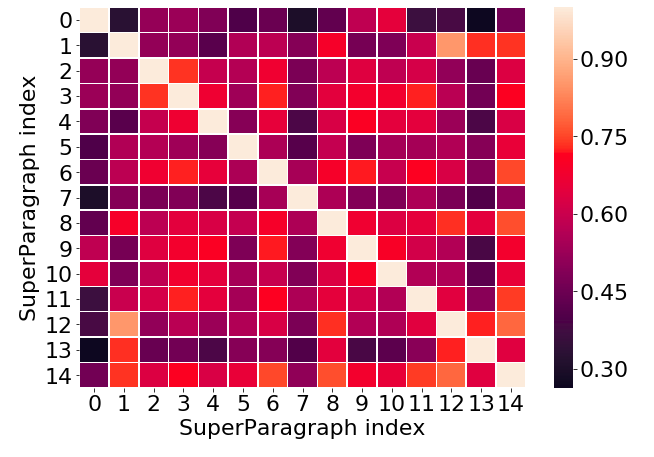
\includegraphics[width=0.49
    \textwidth]{figures/similarity_heatmap.png}
    \caption{Inter \texttt{SuperParagraph} similarity heatmap}
    \label{similarity_heatmap}
\end{figure}

\texttt{SuperParagraph 0}:\\
\textit{Your task is to act as an advisor to an official within the science  ministry. You are advising an official on the issues below. 
The official  is not an expert in the area, but you can assume they are a generally  informed reader.\\
They are interested in the best supported claims in the  documents. Produce a summary of the best supported claims you find and explain why you think they are.\\
Note you are not being asked to "create your own argument" or  "summarise everything you find" but rather, make a judgement about which  claims have the strongest support.}

\texttt{SuperParagraph 13}:\\
\textit{CONCLUSION:\\
Currently, glyphosate dominates crop weed control in soybean, maize,  canola and cotton in North and South America. Consequently, throughout  large areas, glyphosate reliance without diversity in weed control  practices is a strong selection pressure favoring the evolution and  eventual domination of glyphosate-resistant weed populations.}
\newpage
\texttt{SuperParagraph 1}:\\
\textit{INTRODUCTION :\\
Glyphosate  is the active ingredient in Roundup agricultural herbicides and other  herbicide formulations that are widely used for agricultural, forestry,  and residential weed control.\\
It is one of the most widely-used weedkillers in the  world, used by farmers, local government and gardeners, as well as  sprayed\\
extensively on some genetically modified crops imported into  Europe for use as animal feed.\\
Glyphosate,  N-(phosphonomethyl)glycine, is the most extensively used herbicide in  the history of agriculture. Weed management programs in glyphosate  resistant (GR) field crops have provided highly effective weed control,  simplified management decisions, and given cleaner harvested products}

\texttt{SuperParagraph 12}:\\
\textit{6.Glyphosate effects on diseases of plants\\
Glyphosate, N-(phosphonomethyl)glycine, is the most extensively used  herbicide in the history of agriculture. Weed management programs in  glyphosate resistant (GR) field crops have provided highly effective  weed control, simplified management decisions, and given cleaner  harvested products. However, this relatively simple, broad-spectrum,  systemic herbicide can have extensive unintended effects on nutrient  efficiency and disease severity, thereby threatening its agricultural sustainability.  Given that  recommended doses of glyphosate are often many times higher than needed  to control weeds, we believe the most prudent method to reduce the  detrimental effects of glyphosate on GR crops will be to use this  herbicide in as small a dose as practically needed. Such a frugal  approach will not only curtail disease predisposition of GR crops, but  will also benefit the grower and the 
environment.}

We also plotted the time evaluation of inter \texttt{Superparagraph} similarity. In Figure \ref{para_similarity}, each picture shows the evolution in time of the similarity between one \texttt{SuperParagraph} and all \texttt{SuperParagraphs}. The zero values at the beginning indicate that this \texttt{SuperParagraph} was not created yet.

\begin{figure}[htp]
    \centering
    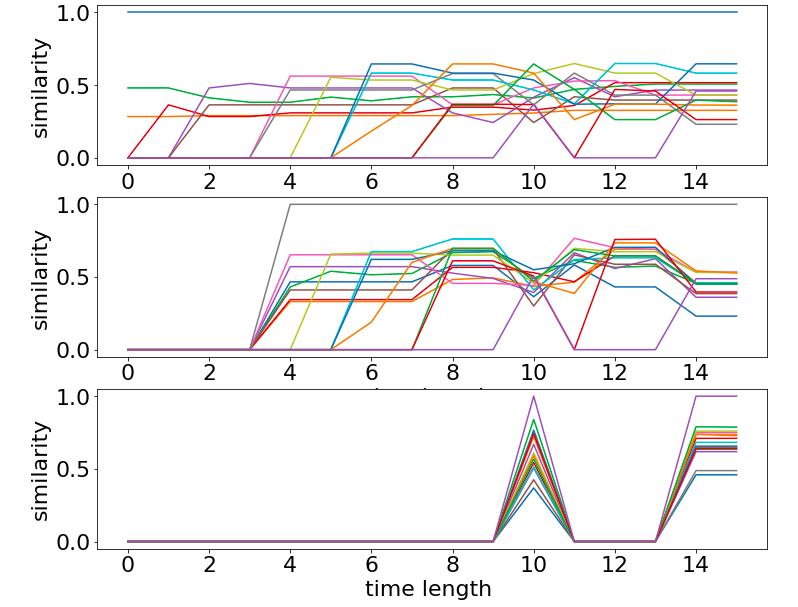
\includegraphics[width=0.49\textwidth]{figures/para_similarity.png}
    \caption{Inter \texttt{SuperParagraph} Similarity through time}
    \label{para_similarity}
\end{figure}



\section{Conclusion}
Compared with previous tools we were based on, we created \texttt{WindowOperation} in order to apply semantic analysis on our tool, and a better time interval will help us to analyze users' data easier. In addition, we tested several pre-trained models and found that sent2vec model has the best performance in our dataset. We can use it to analyze the similarity between \texttt{SuperParagraph} pairs to see if they are related, or apply it to different authors' \texttt{WindowOperations}. We can then obtain the slope of linear model that fits the similarity of authors' \texttt{WindowOperations} for hints on the collaborators' writing behavior.  

Regarding the heuristics implemented for the pad we could see an improvement by redefining the scores that were introduced previously so that they considered only the operations in the last window, as the latter operations are no longer averaged over the total pad and we can see their effect more clearly.

We defined some new measurements regarding the lengths of the \texttt{Paragraphs} and \texttt{SuperParagraphs} (that usually correspond with text lines and text paragraphs, respectively), but with the current timewindow implementation we were not able to reach any conclusion. However, we saw that these measures could potentially give us some interesting insights on how the pad's structure changes in time, suggesting that it may be worth it to explore them further.

\section{Future work}
There are several constrains in our study, mainly due to the limitation of valid data. Besides, the functions defined in our system could be improved by adjusting the parameters with more precision. There are several aspects of the tool in which further work can be carried out, the main ones being:
\begin{itemize}
    \item \textbf{WindowOperation}: The code could be refactored so that the current implementation of WindowOperations is reused for computing pad heuristics in a defined time window. We could also consider reaching a balance between constant-length windows (the approach that we used) and windows that have a length proportional to each Pad's total length as, for instance, in some cases some students may work (or type) faster than others and finish the task earlier.
    \item \textbf{Pad similarity slope}: it could be interesting to discover whether the similarity slope contributes to users' collaborative behavior and try to correlate it with document equality evaluation. Based on those results, we could evaluate whether it would be useful to apply machine learning method to predict the collaborative behavior based on these values.
    \item \textbf{Collaborative behavior pattern}: Analyzing users' collaborative behavior is our main target, as we would like to be able to identify common patterns in order to identify successful collaboration strategies or even predict how much longer will the students take to finish the task. How can we find a way to represent the behavior based on all the metrics we compute is a complex task and could be the main research direction for the future work.
    \item \textbf{Paragraphs and SuperParagraphs tracking}: We implemented paragraph IDs because we were interested in tracking how specific paragraphs could be shifted down by inserting new paragraphs on top, or on how paragraphs were merged and split. However, the paragraph IDs computed seem overly complex. To be able to track specific paragraphs or superparagraphs in the future, the way how we compute this IDs should be improved so that the analysis is more accurate. 
\end{itemize}

% \section{File Structure}
%   \lei{Explain the new added files (Lei)}
%   \lucia{Update explaining run\_analysis etc (Lucia) *}


% \section{Discussion}
%   \todo[inline]{}

% \section{Conclusion}
%   \todo[inline]{}
% \newpage
% \clearpage
\bibliographystyle{unsrt}
\bibliography{refs}

\end{document}
